\documentclass[11pt]{article}
\usepackage[utf8]{inputenc}

% --- Packages ---
\usepackage[usenames, dvipsnames]{color} % Cool colors
\usepackage{enumerate, amsmath, amsthm, amssymb, mathrsfs, algorithm, algpseudocode, pifont, subfig, fullpage, csquotes, dashrule, tikz, bbm, booktabs, bm, hyperref, wasysym}
\usepackage{blindtext, microtype, graphicx, wrapfig, enumitem, fancyhdr, index}
\usepackage[framemethod=TikZ]{mdframed}
\usepackage[numbers]{natbib}
\usepackage[normalem]{ulem}

% --- Misc. ---
\hbadness=10000 % No "underfull̆ hbox" messages.
\setlength{\parindent}{0pt} % Removes all indentation.

% -- Commands --
% Dynamically sized mid bar.
\newcommand{\bigmid}{\mathrel{\Big|}}

% ---- Colors and Notes ----
% ---- Colors and Notes ----
\definecolor{dblue}{RGB}{98, 140, 190}
\definecolor{dmblue}{RGB}{169, 193, 219}
\definecolor{dlblue}{RGB}{216, 235, 255}
\definecolor{dred}{RGB}{195, 112, 113}
\definecolor{dorange}{RGB}{230, 169, 132}
\definecolor{dgreen}{RGB}{83, 127, 85}
\definecolor{dmgreen}{RGB}{118, 167, 125}
\definecolor{dlgreen}{RGB}{154, 195, 157}
\definecolor{dtan}{RGB}{221, 215, 200}
\definecolor{dpink}{RGB}{207, 166, 208}
\definecolor{dyellow}{RGB}{255, 248, 199}
\definecolor{dgray}{RGB}{46, 49, 49}

% Lights
\definecolor{dlblue}{RGB}{169, 193, 219}
\definecolor{dlgreen}{RGB}{154, 195, 157}
\definecolor{dyellow}{RGB}{246, 240, 223}


% URL
\newcommand{\durl}[1]{\textcolor{dblue}{\underline{\url{#1}}}}
\newcommand{\tx}[1]{\text{#1}}

% Circled Numbers
\newcommand*\circled[1]{\tikz[baseline=(char.base)]{\node[shape=circle,draw,inner sep=0.7pt] (char) {\footnotesize{#1}};}}
% From: http://tex.stackexchange.com/questions/7032/good-way-to-make-textcircled-numbers

% Under set numbered subset of equation
\newcommand{\numeq}[3]{\underset{\textcolor{#2}{\circled{#1}}}{\textcolor{#2}{#3}}}

\newcommand{\dnote}[1]{\textcolor{dblue}{Dave: #1}}

% ---- Abbreviations -----
\newcommand{\tc}[2]{\textcolor{#1}{#2}}
\newcommand{\ubr}[1]{\underbrace{#1}}
\newcommand{\uset}[2]{\underset{#1}{#2}}
\newcommand{\eps}{\varepsilon}
\newcommand{\KL}[2]{D_{\text{KL}}\left(#1 \mid \mid #2\right)}
\newcommand{\bKL}[2]{D_{\text{KL}}\left(#1 \bigmid \bigmid #2\right)}

% Typical limit:
\newcommand{\nlim}{\underset{n \rightarrow \infty}{\lim}}
\newcommand{\nsum}{\sum_{i = 1}^n}
\newcommand{\nprod}{\prod_{i = 1}^n}

% Add an hrule with some space
\newcommand{\spacerule}{\begin{center}\hdashrule{2cm}{1pt}{1pt}\end{center}}

% Mathcal and Mathbb
\newcommand{\mc}[1]{\mathcal{#1}}
\newcommand{\indic}{\mathbbm{1}}
\newcommand{\bE}{\mathbb{E}}

\newcommand{\longra}{\longrightarrow}
\newcommand{\longla}{\longleftarrow}
\newcommand{\ra}{\rightarrow}
\newcommand{\la}{\leftarrow}

% argmin, argmax.
\DeclareMathOperator*{\argmin}{arg\,min}
\DeclareMathOperator*{\argmax}{arg\,max}

% Quick Matrix.
\newcommand{\mat}[1]{\begin{bmatrix}#1\end{bmatrix}}

% ---- Figures, Boxes, Theorems, Etc. ----

% Basic Image
\newcommand{\img}[2]{
\begin{center}
\includegraphics[scale=#2]{#1}
\end{center}}

% Put a fancy box around things.
\newcommand{\dbox}[1]{
\begin{mdframed}[roundcorner=4pt, backgroundcolor=gray!5]
\vspace{1mm}
{#1}
\end{mdframed}
}

%  --- PROOFS ---

% Inner environment for Proofs
\newmdenv[
  topline=false,
  bottomline=false,
  rightline = false,
  leftmargin=10pt,
  rightmargin=0pt,
  innertopmargin=0pt,
  innerbottommargin=0pt
]{innerproof}

% Proof Command
%\newenvironment{dproof}{\begin{proof} \text{\vspace{2mm}} \begin{innerproof}}{\end{innerproof}\end{proof}\vspace{4mm}}
\newenvironment{dproof}[1][Proof]{\begin{proof}[#1] \text{\vspace{2mm}} \begin{innerproof}}{\end{innerproof}\end{proof}\vspace{4mm}}


% Dave Definition
\newcounter{DaveDefCounter}
\setcounter{DaveDefCounter}{1}

\newcommand{\ddef}[2]
{
\begin{mdframed}[roundcorner=1pt, backgroundcolor=white]
\vspace{1mm}
{\bf Definition \theDaveDefCounter} (#1): {\it #2}
\stepcounter{DaveDefCounter}
\end{mdframed}
}

% Block Quote
\newenvironment{dblockquote}[2]{
\begin{blockquote}
#2
\vspace{-2mm}\hspace{10mm}{#1} \\
\end{blockquote}}

% Algorithm
\newenvironment{dalg}[1]
{\begin{algorithm}\caption{#1}\begin{algorithmic}}
{\end{algorithmic}\end{algorithm}}

% Dave Table
\newenvironment{dtable}[1]
{\begin{figure}[h]
\centering
\begin{tabular}{#1}\toprule}
{\bottomrule
\end{tabular}
\end{figure}}

% For numbering the last of an align*
\newcommand\numberthis{\addtocounter{equation}{1}\tag{\theequation}}


\newtheorem{assumption}{Assumption}
\newtheorem{conjecture}{Conjecture}
\newtheorem{corollary}{Corollary}
\newtheorem{claim}{Claim}
\newtheorem{example}{Example}
\newtheorem{lemma}{Lemma}
\newtheorem{proposition}{Proposition}
\newtheorem{remark}{Remark}
\newtheorem{theorem}{Theorem}

\begin{document}
\title{CVPR 2019 Notes \\ \Large{Long Beach, CA, USA}}
\author{Shuai Chen \\ \durl{shuaic92@gmail.com}}
\date{June 2019}

\maketitle
\tableofcontents
\newpage

This documents contains notes I took during CVPR 2019 conference in Long Beach, CA, USA. My motivation of making this document came from the inspiration of David Abel\footnote{\durl{http://david-abel.github.io}}. Please feel free to distribute it as well as correcting my typos and mistakes. My email is \durl{shuaic92@gmail.com}.

\section{Conference Highlights}
This was my first time took part in such an awesome academic conference. Most of my time spent in Deep Learning \& Computational Photography related topics. However, I would also update some topics that I found interesting.
\begin{enumerate}
    \item Around 10,000 people attend this year's conference. About 1300 papers were accepted in CVPR 2019. Reports saying number of attendees projected in 2035 will be over 1 million :). See Figure \ref{fig:Conf_HL1}.
    \begin{figure}[h!]
        \centering
        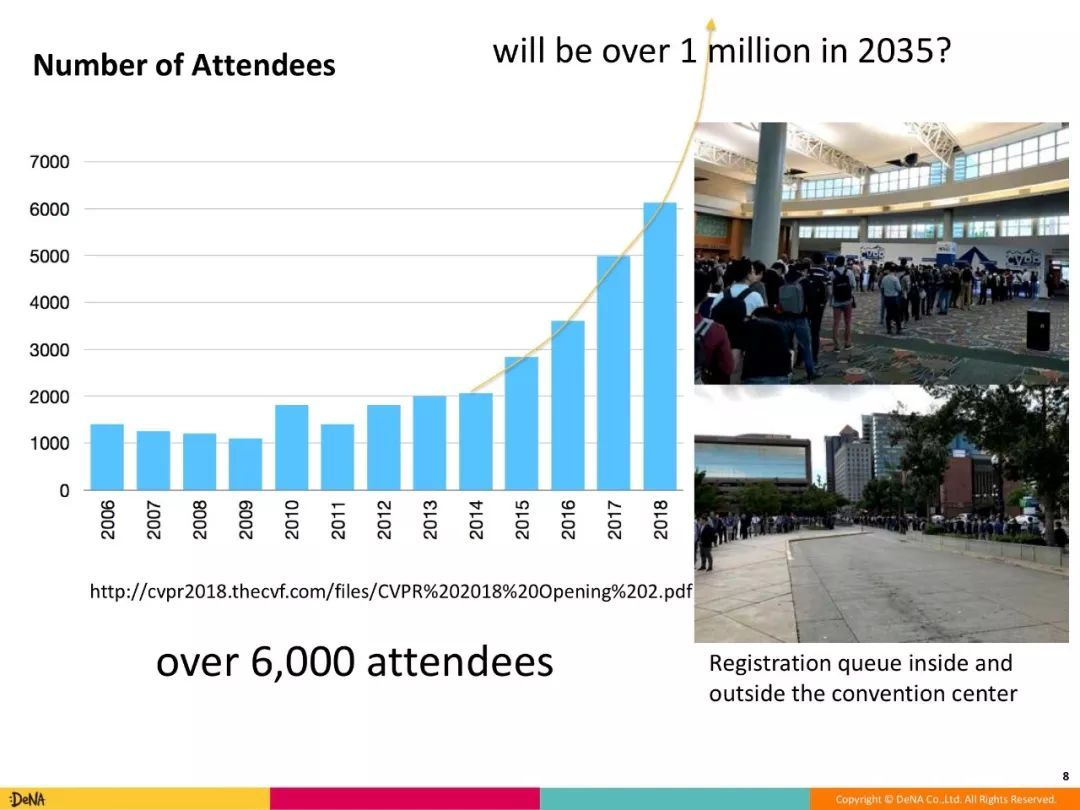
\includegraphics[width=0.5\textwidth]{images/Image1.jpeg}
        \caption{projection of attendees to reach 1 million by 2035}
        \label{fig:Conf_HL1}
    \end{figure}
    
    \item Comparing to last year, the number of papers accepted in CVPR 2019 increased about 30\%. However, due to the fact that the number of papers submitted this year has increased 56.2\%, thus the paper acceptance rate reduced 4\% this year. See Figure \ref{fig:Conf_HL2}.
    \begin{figure}[ht!]
        \centering
        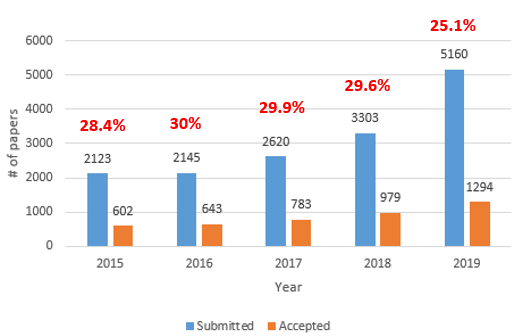
\includegraphics[width=0.5\textwidth]{images/Image2.png}
        \caption{papers acceptance rate is 4\% lower in CVPR 2019}
        \label{fig:Conf_HL2}
    \end{figure}
    
    \newpage
    \item Some of hot keywords in CVPR 2019 submission: Image, detection, 3d, object, video, segmentation, adversarial, recognition, visual. See Figure \ref{fig:Conf_HL3}
    \begin{figure}[ht!]
        \centering
        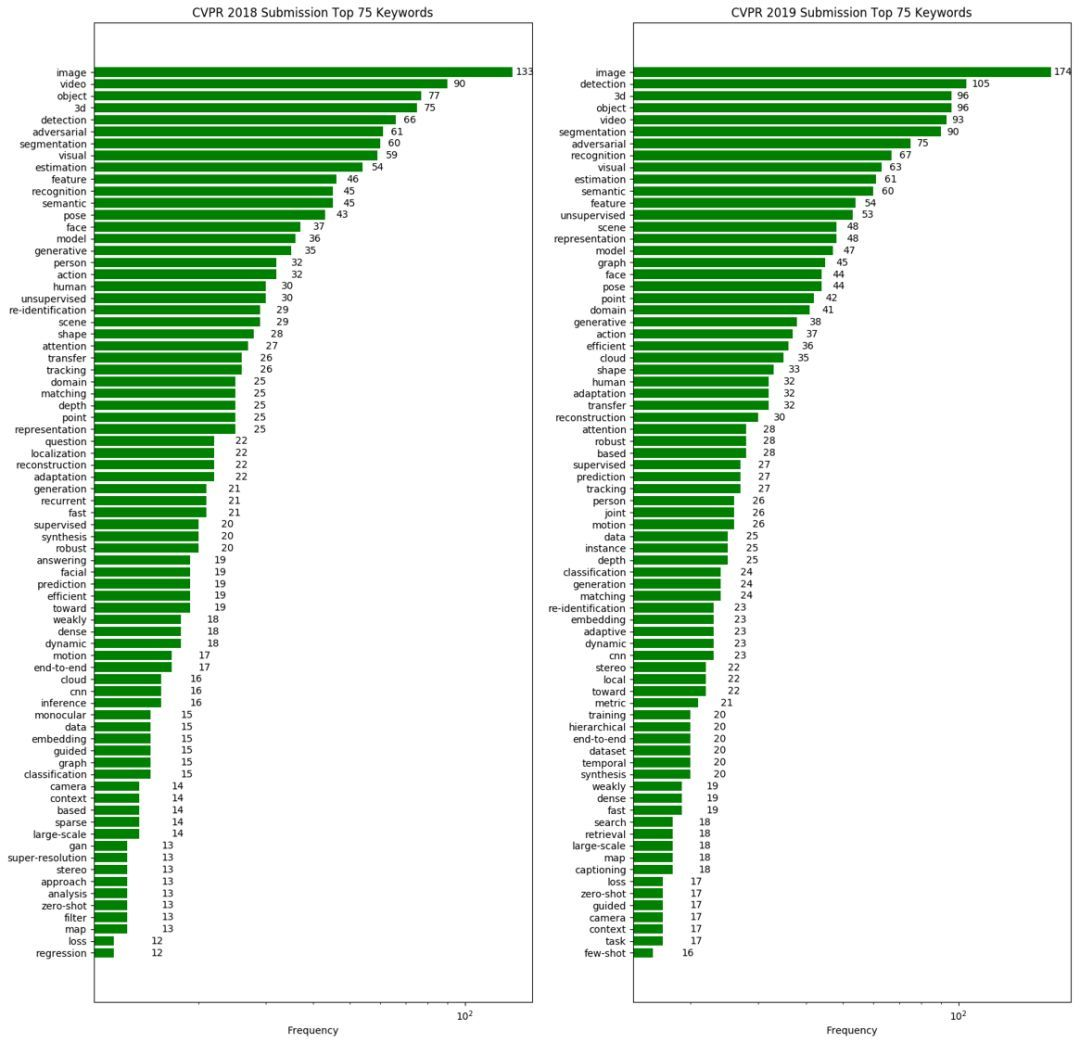
\includegraphics[width=0.9\textwidth]{images/Image3.jpeg}
        \caption{hot submission keywords CVPR 2018 vs. CVPR 2019}
        \label{fig:Conf_HL3}
    \end{figure}
    
    \item More Meta-learning, One-shot/Few-shots learning, Graph Neural Networks papers started to emerge this year.
    \item It's great to see a lot of fast pace improvement towards real-life low level image processing field.
    \item Network Architecture Search was also another very popular topic. Great to see a burst of diverse solutions in this field.
    \item Generative Adversarial Network was a hot topic again. Exciting progress were made again this year.
\end{enumerate}{}

% ------------
% -- Sunday --
% ------------
\newpage
\section{Sunday June 16th: Tutorials \& Workshops}
Caught up part of Deep-Vision workshop. I was a little bit confused on overwhelming tutorials and workshops. I also spent a lot of time trying to find the correct room. So first day's note was not really good. Please feel free to contact me and add some notes.

\subsection{Workshop: Deep-Vision}
\subsubsection{Topic: AI on Medicine, Speaker: Serena Yeung}
Arrived at the end of the talk on this topic. She talked about Learning from few labeled training examples \\
\textbf{Learning to learn from noisy web videos (CVPR2017)}\newline
{\bf Idea:} Proposed a Reinforcement learning-based method for learning data labeling form noisy web videos. Result is able to learn domain-specific knowledge, and label data for new classes while avoiding semantic drift.\\
\\
\begin{figure}[]
    \centering
    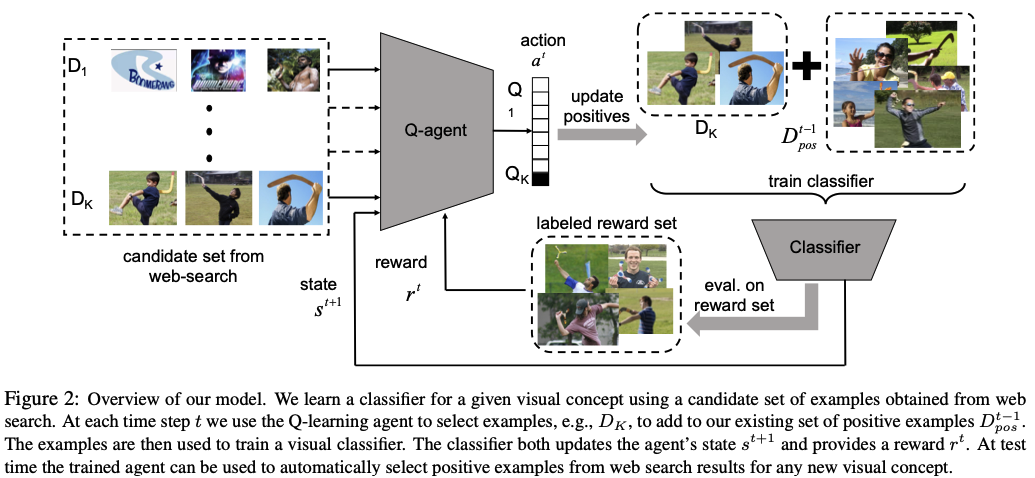
\includegraphics[width=1\textwidth]{images/Image4.png}
    \label{fig:Conf_D1_1}
\end{figure}\\
{\bf Terminology:} \textit{candidate set:} noisy search result. \textit{reword set:} a set of examples annotated with the presence or absence of the target class.\\
\\
\textbf{Temporal Modular Networks for Retrieving Complex Compositional Activities in Videos (ECCV2018)}\\
\\
\textbf{Neural Graph Matching Networks for Fewshot 3D Action Recognition (ECCV2018)}\\
\\
Talked about Towards full realization of an AI-assisted hospital: Integration of multimodal data sources. \\
Talked about Jointly Learning Energy Expenditures and Activities using Egocentric Multimodal Signals (CVPR 2017) \\
Will add a short paper summary here... \\

\subsubsection{Topic: Video Re-Id, Speaker: Prof. Dr. Laura Leal-Taixé}
Tractor++ (reId+CMC)\\
CMC = motion camera model
\subsubsection{Topic: Video Super-resolution, Speaker: Prof. Dr. Laura Leal-Taixé}
Designed new Temporal Loss to improve video SR performance. Great results.
\subsubsection{Topic: Google Brain Pierre Sermanet: Self-Supervision and Play}
-Label Free\\
-Time-Contrastive Networks (TCN)\\
-Object-contrastive Networks\\



% ------------
% -- Monday --
% ------------
\newpage
\section{Monday June 17th: Tutorials \& Workshops}
\subsection{Workshop: Computational Photography}
Light Field Super-Resolution A Benchmark\\

Low Rank Poisson Denoising(LRPD)\\

\subsubsection{Professor Peyman Milanfar: Computation + Photography How the mobile phone became a camera}
    - Modern Mobile Imaging: Burst Photography. ?Burst Video?\\
    - Classical camera pipeline -demosaicing (Merging)\\
    - Replace demosaicing with multiple frames\\
    - Pixel Shifting\\
    - Merge: Nonlinear Kernel Regression\\
    - Merge High-res Grid -> up to 2x\\
    - Source of motion imaging: 1. OIS, 2. (rough) alignment by (Natural) Physiological Tremor\\
    - use OIS simulate tremor!!!!\\
    - Aliasing + Phase diversity -> Multi-frame Super-res\\
    - Visual System also appears to do super-resolution\\
    - Handheld Multi-Frame Super-Resolution (Why not using GAN)\\
    - Zoom Use Case: to zoom more: Upscale SISR, using RAISR\\
    - Other Challenge in Computational Photography: Curation (NIMA for Aesthetic Quality, NIMA for Technical Quality)\\
    - Camera Understand the Scene and the User\\
    - Night Sight Mode: Super Night Sight on Merge Methods. ML on White Balance\\

\subsubsection{SuperSR}
    - Overfitting in Super Resolution\\
    - MixUp: Data Synthesis with Learned Degradation\\
\subsubsection{Denoising}
    - Hanyang University\\
    - Hierarchical Structure\\
    - Iterative down-sampling and up-sampling\\
    - Down-up Block\\
    - Noise Level\\
\subsubsection{Style-based GAN: Kerras}
    - Progressive GAN\\
    - BigGAN\\
    - Pose-Guided Face Rotation\\
    - Mask-Guided Portrait Editing\\

\subsubsection{Image Coloring Challenge}

\subsubsection{Opportunity Chiuman Ho, Director of AI: Imaging in the Dark}
    - l1 > l2 since l2 penalize a lot on large loss\\
    - Feature Loss\\

\subsubsection{Blind Deconvolution: Professor Paolo Favaro}
    -Learning to Extract Flawless Slow Motion from Blurry Videos CVPR 2019.\\
    -f = k * u + n\\
\subsubsection{EDVR}

\subsubsection{Towards Versatile Image Restoration: Chen-Change LOY}
...

% ------------
% -- Tuesday --
% ------------
\newpage
\section{Tuesday June 18th: Main Conference Day 1}
\subsection{CVPR Main Day 1}
Oral:\\
\subsubsection{GNN}
\begin{enumerate}
    \item Few Shot Learning: EGNN
    \item Few Shot Classification
\end{enumerate}
\subsubsection{Kervolutional Neural Network}
    1. Introduce nonlinearity in convolution\\
\subsubsection{Relu with high confident}
    1. Adversarial confidence enhanced training (ACET)\\
\subsubsection{Structural Sensitivity of DCN to the Directions of FOurier Basis Functions}
\subsubsection{neural rejuvenation}
\subsubsection{On the Structural Sensitivity of Deep Convolution}
\subsubsection{Hardness aware Deep Metric Learning}
\subsubsection{Auto-Deeplab: NAS for Semantic Image Segmentation}
\subsubsection{Learning Loss for Active Learning }
    1. Active Learning \\
\subsubsection{Striking the Right Balance With Uncertainty}
\subsubsection{Auto Augment}
\subsubsection{Zero Shot}
    1. Domain Loss \\
    2. Triplet Loss \\
    3. Semantic Loss \\
\subsubsection{Zero-shot Task Transfer}
    1. Regress the unknown zero-shot task \\
\subsubsection{C-MIL: sWeakly Supervised Object Detection}
    1. Solve non-convex loss function problem \\
\subsubsection{Weakly Supervised Learning of Instance Segmentation}
    1. Learning Displacements to Centroid (Find Instance) \\
    2. Learning Class Boundaries (Find Shape) \\
\subsubsection{Attention-Based Dropout Layer for Weakly Supervised Object Localization}
    1. Adversarial Erasing \\
    2. Spatial Attention Transformation \\
    3. Attention-based Dropout layer \\
    4. attention-based, efficient, State of the art localization accuracy \\
\subsubsection{Domain Generalization by Sol Jigsaw Puzzles}
    1. Recognition -> Jigsaw Puzzles \\
    2. Domain Generalization \\
    3. Multitask deep learning model \\
\subsubsection{Transferable Prototypical Networks for Unsupervised Domain Adaptation}
    1. Most methods are cascaded model \\
    2. Multitask into one network \\
    3. Supervised classification loss, class-level discrepancy loss, sample-level discrepancy loss \\
\subsubsection{Blending-target Domain Adaptation}
    1. Source-target domain discrimination, still lack of target domain area \\
    2. Adaptation among Meta-sub-targets \\
\subsubsection{ELASTIC: Improving CNNs with dynamic Scaling Policies}
    {\bf Problem:} CNN image scaling are handcrafted \\
    {\bf Solution:} CNN to learn dynamic scaling policies \\
    {\bf Result:} Consistent improvement \\
\subsubsection{ScratchDet: Training Single-Shot Object Detectors From Scratch}
    {\bf Problem:} High Computational cost on ImageNet, Learning bias from classification to detection, inconvenient to change the architecture of network \\
    {\bf Contribution:}  \\
        1. Batch Norm \\
        2. Replace 7x7 by stacking 3x3 3x3... \\
        3. BatchNorm in the backbone key for detection to train from scratch \\
\subsubsection{SFNet: Learning Object-aware Semantic Correspondence}
    {\bf Problem:} Lack of dataset semantic correspondences \\
    {\bf Solution:} 3.Loss functions: Mask consistency, smoothness, and ... \\
    {\bf Result:}  \\
\subsubsection{Deep Metric Learning Beyond Binary Supervision}
    {\bf Problem:} most metric learning are same or not (binary). Population pos and neg are unbalanced \\
    {\bf Solution:}  \\
        1. Log-ratio loss. \\
        2. Dense Triplet Sampling \\
    {\bf Result:} \\
        1. Three retrieval: surpass state of the art \\
\subsubsection{Learning to Cluster Faces on an Affinity Graph}
    {\bf Problem:} Clustering human faces, complex structure are difficult to use kmeans or spectral \\
    {\bf Solution:} Generate Proposal - GCN-Detection - GCN-Segmentation \\
    {\bf Result:} state of the art F-score \\
\subsubsection{C2AE: Class Conditioned Auto-Encoder for Open-Set}
    {\bf Problem:} Open set recognition \\
    {\bf Solution:}  \\
        1. Closed set training \\
        2. Open set training, Decoder \\
        3. Open-set Testing (k-Inference Algorithm) \\
    {\bf Results:} \\
        1. F-measure highest \\
            1. Quantitative Analysis \\
\subsubsection{Samsung: Learning to Quantize Deep Networks by Optimizing}
    {\bf Problem:} Reducing bit-widths while minimizing accuracy drop \\
    {\bf Solution:} Find meaningful dynamic range for quantization \\
        1. Activation Quantizer \\
        2. Weight Quantizer \\
    {\bf Result:}  \\
        1. better than others \\
        2. Heterogeneous training \\
\subsubsection{Transfer Learning for Semantic Segmentation via Hierarchical Region Selection}
    {\bf Problem:} \\
        1. Insufficient real data + a lot of unreal data \\
    {\bf Solution:} \\
        1. Source Image with Weighting Mask \\
        2. Feed in Source \& target domain \\
        3. Use GAN to reduce domain differences \\
\subsubsection{Unsupervised Learning of Dense Shape Correspondence}
    {\bf Problem:} traditional supervised, want unsupervised \\
    {\bf Solutions:} \\
        1. No expensive annotations \\
        2. Geometric Invariants \\
    {\bf Result:} \\
        1. Achieve same result with Supervised \\
        2. Achieve state of the art accuracy without seen label \\
    {\bf Self-supervised Training Regime:} \\
\subsubsection{Unsupervised Visual Domain Adaptation: A Deep Max-Margin Gaussian Process Approach}
    {\bf Problem:} Traditional, learning source \& target distributions. Fail at lack of domain labels -> No guarantee \\
    {\bf Solution:} \\
        1. Source-driven Gaussian Process posterior (H) inference \\
        2. Target domain Max Margin Seperation \\
\subsubsection{Balanced Self-Paced Learning for Generative Adversarial Clustering Network}
    {\bf Problem:}  \\
    {\bf Solution:} Deep GAN Clustering Network \\
        1. Entropy Minimization Loss \\
\subsubsection{Parallel Optimal Transport GAN}
    {\bf Problem}


% ------------
% -- Wednsday --
% ------------
\newpage
\section{Wednsday June 19th: Main Conference Day 2}
\subsection{Photography Oral: (Day2)}
\subsubsection{Photon-Flooded Single-Photon 3D Cameras}
    1. {\bf Problem:} Sunlight disturb Ambient light \\
    2. {\bf Solution:}  \\
        1. Find Optimal Filtering: low distortion, high SNR \\
    3. {\bf Result:} \\
        1. Long Range Low Power 3D Imaging \\
\subsubsection{High Flux Passive Imaging with Single-Photon Sensors}
    1. SPADs \\
    2. {\bf Problem:} Noise PF-SPAD, High Flux fail to catch Photons \\
    3. {\bf Solution:} PF-SPAD Sensor can catch High Dynamic Range \\
    4. {\bf Result:} PF-SPAD: SPADs as General-Purpose, Passive Sensors. \\
\subsubsection{Acoustic Non Line of sight Imaging}
    1. {\bf Problem:} Expensive \\
    2. {\bf Solution:} Acoustic, cheap. Use Wall as mirror. \\
\subsubsection{Steady-State Non Line of Sight Imaging}
    1. {\bf Problem:} Large setup size. Expensive \\
    2. {\bf Solution:} \\
\subsubsection{A Theory of Fermat Paths for Non line of sight shape reconstruction (CVPR19 best paper)}
    1. {\bf Problem:} Non line of sight \\
    2. {\bf Solution:} Scanning the wall \\
        1. Fermat path lengths = discontinuities \\
        2. Fermat path = specula or boundary \\
        3. Add regularization term \\
        4. Optical Coherence Tomography to high resolution \\
    3. {\bf Result:}  \\
        1. High resolution \\
\subsubsection{Projector Photometric Compensation}
    1. {\bf Problem:} Projection distort image \\
    2. Contribution:  \\
        1. CompenNet CNN \\
        2. Premarin method \\
        3. Benchmark \\
    3. {\bf Solution:} \\
        1. Capture Surface image and camera image \\
        2. Train CompenNet \\
    4. {\bf Result:} \\
        1. Surpass State of the art \\
\subsubsection{Bringing a Blurry Frame Alive at High Frame-Rate With an Event Camera}
    1. {\bf Problem:} Event camera likely to capture blur image \\
    2. {\bf Solution:}  \\
        1. Double Integral while feeding in event. \\
        2. Find gradient descent by Fibonacci search \\
    3. {\bf Result:} \\
        1. Sharp Video Sequence \\
\subsubsection{Bringing Alive Blurred Moments}
    1. {\bf Problem:} unsuitable for realtime,Too many unknowns, estimate only in one image \\
    2. {\bf Solution:} \\
        1. Learn Extract motion from a sharp frame sequence \\
        2. Recurrent Video Encoder decoder \\
\subsubsection{Learning to Synthesize Motion Blur}
    1. {\bf Problem:} Motion During Exposure Causes Blur, accidental , Purposefully  \\
        1. Optical Flow Blur unwanted object  \\
    2. {\bf Solution:} Synthetic Motion Blur \\
        1. Train Model to synthesize \\
        2. Could learn occlusion \\
        3. Training Date Generation: \\
            1. Train Frame interpolation network \\
            2. Average for motion blur \\
    3. {\bf Result:} \\
        1. High dB \\
        2. Short Time \\
        3. Handling Complex Motions Better than Optical flow method \\
\subsubsection{Underexposed Photo Enhancement Using Deep Illumination Estimation}
    1. {\bf Problem:} Pixel-wise mapping has limitation \\
    2. {\bf Solution:}  \\
        1. Illumination Map \\
        2. Smoothness loss \\
\subsubsection{Blind Visual Motif Removal From a Single Image}
    1. {\bf Solution:}  \\
        1. 1 encoder, 3 decoders \\
        2. A bunch of losses \\
    2. Test Result \\
\subsubsection{Non-Local Meets Global: an integrated Paradigm for Hyper-spectral Denoising}
    1. {\bf Problem:}  \\
        1. More spectral bands, more computation burden \\
    2. {\bf Solution:}  \\
        1. Non-local similarity and global spectral low-rank property \\
\subsubsection{Neural Rendering in the wild}
    1. {\bf Solution:} Train Neural Render. Multiple stage training \\
\subsubsection{GeoNet: Deep Geodesic Networks for Point Cloud Analysis}

% ------------
% -- Thursday --
% ------------
\newpage
\section{Thursday June 20th: Main Conference Day 3}
\subsection{Low-level \& Optimization Oral: (Day3)}
\subsubsection{Unprocessing Images for Raw Denoising}
{\bf Problem:} Traditional: Synthetic Data Denoising. Not Real \\
        1. Real Camera Data: a high quality denoising dataset for smartphone cameras: best is BM3D \\
        2. SRGB image + additive Gaussian noise \\
        3. Raw + noise\\
{\bf Solution:} \\
        1. Find Unprocessed Data \\
        2. Raw sensor data $\ra$ Denise \& demosaic $\ra$ Color Correction $\ra$ gamma compression $\ra$ Tone mapping $\ra$ sRGB image \\
        3. Unprofessional images reverse the pipeline \\
        4. Realistic Training data\\
{\bf Results:} \\
        1. Best in DND\\
{\bf Takeaways:} \\
        1. Realistic Training data \\
        2. Unprocessing data $\ra$ better training results \\
\subsubsection{Residual Network for Light field image super resolution}
    1. {\bf Problem:} \\
        1. 
    2. {\bf Solution:} \\
        1. Extract subpixel in four direction \\
        2. Combine with ... \\
    3. {\bf Result:} \\
        1. Best result in Buddha and Mona \\
        2. Surpass EDSR \\
\subsubsection{Modulating image restoration with Continual Levels via adaptive feature Modification Layers}
    1. {\bf Problem:} \\
        1. Degradation levels of real world image are continuous \\
        2. Deep restoration is discontinuous \\
        3. Cannot train large model to handle all degradation levels \\
    2. {\bf Solution:} \\
        1. Propose AdaFM (Adaptive Feature Modification layer) \\
        2. 1. Train basic layer, 2. Insert AdaFM, 3.... \\
        3. 7x7 filter achieve better then 5x5 3x3. \\
        4. Arbitrary Result for Style transfer \\
\subsubsection{Second-Order Attention Network for Single Image Super-Resolution}
    1. {\bf Problem:} neglect rich feature correlations (most work) \\
    2. {\bf Solution:} \\
        1. Attention based mechanism \\
            1. Spatial Attention \\
            2. Channel Attention \\
        2. Use Spatial \& Channel attention simultaneously \\
            1. Second-order attention network SAN \\
            2. Use Newton Schulz iteration to solve eigenvalue decomposition (is not well supported on GPU platform) \\
    3. {\bf Result:} \\
        1. Better than VDSR \\
\subsubsection{Devil is in the Edges: learning Semantic Boundaries from noisy annotation}
    1. {\bf Problem:} \\
        1. Boundary annotation imprecise, current SOTA \\
        2. Annotation Hard \\
    2. {\bf Solution:} \\
        1. Propose STEAL \\
        2. Semantic Thinning Edge Alignment layer \\
    3. {\bf Result:} \\
        1. SBD dataset achieve state of the art \\
        2. CITYSCAPES: 4.2% better \\
    4. Dataset Refinement, annotate coarse masks fast, refine masks with STEAL \\
\subsubsection{Path-Invariant Map Networks}
    1. {\bf Problem:} \\
        1. Invariant map problem \\
    2. {\bf Solution:} \\
        1. Path Invariance provides a regularization for training neural networks \\
        2. Supervised loss + unsupervised loss \\
    3. {\bf Result:} \\
        1. Leverage additional training data \\
        2. Fuse attention... \\
        3. ... \\
\subsubsection{FilterReg: Robust and Efficient Point-set registration}
    1. {\bf Problem:} \\
        1. Iterative Closest Point: relatively fast but sensitive to.. \\
    2. {\bf Solution:} \\
        1. Filter-based Correspondence \\
    3. {\bf Result:}  \\
        1. 40ms runtime \\
        2. 30% faster than SOTA GPU method GMMTree \\
        3. Feature-based Registration \\
\subsubsection{Probabilistic Permutation Synchronization Using the Riemannian Structure of the Birkhoff Polytope}
    1. {\bf Problem:} \\
        1. Synchronization of Multiview Correspondences \\
        2. Correct Mistakes + Estimate Match Confidence \\
    2. {\bf Solution:} \\
        1. Encode Pairwise Correspondence\ as total permutations \\
        2. Minimize the cycle consistency loss over the entire (hyper-) graph \\
        3. Propose Birkhoff Riemannian Langevin Monte Carlo \\
    3. {\bf Result:} \\
        1. Achieve state of the art of L-BFGs algorithm \\
\subsubsection{Lifting Vectorial Variation Problems:}
    1. {\bf Problem:} \\
        1. Global energy minimization \\
    2. {\bf Solution:} \\
    3. OK I gave up \\
\subsubsection{A Sufficient Condition for Convergences of Adam and RMSProp}
    1. {\bf Problem:} \\
    2. {\bf Solution:} \\
        1. Modify Adam to Generic Adam \\
        2. Weighted AdaEMA \\
        3. Propose Sufficient condition \\
\subsubsection{Guaranteed Matrix Completion Under Multiple Linear Transformation}
    1. {\bf Problem:} \\
        1. Significant low-rank structure appears under some transformations \\
        2. The conventional theoretical analysis for guarantee is no longer suitable \\
    2. {\bf Solution:} \\
        1. Propose generalization the problem as Matrix Completion under Multi linear-Transformations MCMT \\
        2. The upper-bound of the reconstruction error is linearly controlled by the condition number of the transformations \\
\subsubsection{MAP inference via Block-Coordinate Frank-Wolfe Algorithm}
    1. {\bf Problem:} \\
\subsubsection{A convex relaxation for multigraph matching}
    1. {\bf Problem:} \\
        1. Multi-graph matching \\
        2. Cycle consistency matching \\
    2. {\bf Contribution:} \\
        1. Partial matching \\
        2. Quadratic costs \\
        3. Higher order costs \\
        4. Optimization: LP formulation \\
        5. Convergence: Lower bounds \& optimization gap \\
        6. Scalability: Linear \\
    3. {\bf Result} \\

% ------------
% --- Todo ---
% ------------
\newpage
\end{document}

